\documentclass[10pt]{article}
\usepackage[margin=20mm]{geometry}
\usepackage{amsmath,amssymb,amsthm,bm,graphicx,booktabs,array,float,microtype}
\usepackage[hidelinks]{hyperref}
\usepackage{cite}
\newcommand{\R}{\mathbb R}
\newcommand{\diag}{\operatorname{diag}}
\newcommand{\norm}[1]{\lVert #1\rVert}
\newcommand{\ket}[1]{\lvert #1\rangle}
\newcommand{\lchsnode}{\eta}
\newcommand{\lchsshift}{\theta}
\renewcommand{\theequation}{S\arabic{equation}}
\setlength{\emergencystretch}{2em}
\title{Technical supplement:\\Quantum Calibration of Local-Volatility Surfaces\\from Sparse Option Quotes}
\author{Kentaro Hoshisashi\\ \small Department of Computer Science, University College London}\date{}
\begin{document}\maketitle
The main paper presents the financial problem, resulting implied-volatility
surfaces and price comparisons. This supplement retains the discretisation,
derivations, quantum construction and numerical diagnostics needed to reproduce
and assess those claims. The new main-paper surfaces are evaluated at four
actual maturities. The earlier numerical benchmark and its diagnostic figures
are retained separately, with their original model and execution provenance.
\tableofcontents
\section{New measured multi-expiry experiment}
The main paper adds a measured hybrid calibration to the larger archived
financial benchmark. These are separate experiments. The new circuit has
$N=4$ interior nodes, two basis functions with centres $(-0.55,0.55)$ and
width $0.85$, and maturities $(0.5,1)$ years. Four irregular quotes per maturity
are used. The exact same-grid target has coefficients $(0.75,0.25)$ and
$(0.25,0.75)$. It isolates circuit, quadrature and sampling errors. The larger
archived benchmark instead uses $M=4$ and fine-grid target generation.

\subsection{Product of successful propagation blocks}
Let $U_s$ have successful block $\widetilde P_s/(e^{\lchsshift\Delta_s}\alpha)$.
Allocate a fresh LCU register to every interval and use the same system register.
Since subsequent operators do not act on a previous interval's LCU register,
projection of all of them onto zero gives
\begin{equation}
 \left(\prod_{r=1}^s\langle0|_{a_r}\right)U_s\cdots U_1
 \left(\prod_{r=1}^s|0\rangle_{a_r}\right)
 =\frac{\widetilde P_s\cdots\widetilde P_1}{e^{\lchsshift T_s}\alpha^s}.
\end{equation}
Failed branches cannot re-enter a previously successful subspace, since that
register is never reused. There is no intermediate measurement or replacement
with a classically computed state.

\subsection{Observation and residual measurement}
Pad the quote map to an $N\times N$ matrix $W_s$ and its target to an
$N$-vector $y_s$. This prototype requires $q_s\leq N$.
For $B=W_s/\gamma_s$, $\gamma_s=\max(1,\norm{W_s}_2)$, the circuit uses
\begin{equation}
 U_B=\begin{pmatrix}B&\sqrt{I-BB^\dagger}\\
 \sqrt{I-B^\dagger B}&-B^\dagger\end{pmatrix}.
\end{equation}
The implementation checks unitarity numerically. With
$a_s=\norm{v_0}_2e^{\lchsshift T_s}\alpha^s\gamma_s$ and
$d_s=\norm{y_s}_2$, prepare the residual branch with amplitudes
$\sqrt{a_s/(a_s+d_s)}$ and $\sqrt{d_s/(a_s+d_s)}$.
Controlled preparation of the propagated state and $y_s/d_s$, a relative
minus sign and inverse branch preparation produce successful residual
$(W_s\widetilde v_s-y_s)/(a_s+d_s)$.
The all-zero ancillary frequency therefore estimates the squared residual,
with its known scale retained. The supplied financial target has $d_s>0$.
A general zero-target instance would need its trivial separate branch.

\subsection{Search, replication and interval reporting}
Both matrix and measured objectives use the same bounded pattern search.
Starting at four coefficients equal to $0.5$, two sweeps test the incumbent
and positive/negative steps of $0.25$ along four coordinate directions and
two within-interval tilt directions. Coordinates are clipped to $[0,1]$ and
duplicate candidates are removed. Ties retain the earlier candidate, with
the incumbent tested first. The finite search does not claim global optimisation.

The paper configuration uses $J=8$, cutoff $12$, and respectively $2^{18}$
and $2^{22}$ repetitions per maturity per candidate, each with seeds
$101,202,303$. Only backend finite-shot counts enter coefficient decisions.
Independent matrix and statevector checks occur outside the search.
Final smile plots are matrix re-evaluations at the selected coefficients.
The raw measurement record separately shows what was observed. Held-out
errors use the known synthetic target only for reporting.

After selection, a fresh evaluation supplies the reported interval. Each
maturity uses a Clopper--Pearson binomial interval with tail probabilities
$0.05/(2S)$. Scaling and averaging these intervals gives a conservative
95\% interval for the final finite-circuit objective by a union bound.
For zero observed successes, the upper endpoint remains positive. Per-call
Wald standard errors are also logged as descriptive approximations, but are
not used to certify a zero loss. Calibration and independent-check shot/gate
totals have separate fields. Transpiled $u$/CNOT circuits are exported
in QPY format. Counts assume all-to-all connectivity without error correction.

The resource sweep uses cutoff $4$ for $J\leq8$ and $32$ otherwise, varying
$N,J$ and the number of maturity intervals. This is a gate-size diagnostic.
The $J=8$ calibration uses cutoff $12$. Both cutoffs are recorded explicitly.
An additional matrix-only quadrature sweep varies cutoff and term count
together. Its accuracy figures are not hardware measurements.

\section{Archived financial calibration problem}
\subsection{Financial normalisation and parameterisation}
With deterministic rates and proportional dividend yield, let $D(T)$ and $F(T)$ be the discount factor and forward. Write $k=K/F(T)$ and $c(T,k)=C(T,K)/(D(T)F(T))$. The forward-normalised equation is
\begin{equation}
 \partial_T c=\tfrac12 a(T,k)k^2\partial_{kk}c,\quad
 c(0,k)=(1-k)^+ . \label{eq:dupire}
\end{equation}
The coefficient $a$ is the local variance evaluated at the corresponding forward-scaled asset price. The zero-carry case is included. Discrete cash dividends, American exercise, stochastic rates, and inconsistent forwards fall outside this model.

On slice $(T_{s-1},T_s]$, set $x=\log k$ and
\begin{equation}
 a_s(x;\xi_s)=a_{\min}+\sum_{j=1}^M\xi_{sj}\phi_j(x),\qquad 0\leq\xi_{sj}\leq1, \label{eq:basis}
\end{equation}
where $a_{\min}=0.01$ and
$\phi_j(x)=0.04[1+\cos(\pi(x-\mu_j)/w)]\mathbf1_{|x-\mu_j|\leq w}$.
The archived financial model uses $M=4$, centres $(-0.6,-0.2,0.2,0.6)$ and $w=0.45$. This is a restricted positive family, not an arbitrary local-variance surface. Compact support makes these functions $C^1$ but generally not $C^2$ at support endpoints. They are not globally finite Fourier polynomials.

\subsection{Boundary lift, observations, and loss}
Use $k\in[k_0,k_{N+1}]=[e^{-1.2},e^{1.2}]$, with fixed boundary values $c(T,k_0)=1-k_0$ and $c(T,k_{N+1})=0$. These are a domain truncation assumption, not exact far-field values at finite strikes. Let $G(k)$ be the affine-in-strike interpolant of these boundary values. The interior homogeneous state is $v=c-G$. Since $G''=0$, the fitted discretisation below has no lift forcing.

For an off-grid quote, $W_s$ contains the two nonnegative piecewise-linear weights in \emph{strike}. Boundary contributions are included before setting $y_s=c_s^{\rm obs}-W_s^{\rm full}G$. Thus $W_s$ need not be a row-selection matrix and $W_s^TW_s$ need not be a projector. The slice loss is
\begin{equation}
 \mathcal L_s(\xi_s)=\frac1{q_s}\norm{\Omega_s(W_s v_s-y_s)}_2^2
 +\lambda\frac{\norm{D_2\xi_s}_2^2}{M-2}, \label{eq:loss}
\end{equation}
with the last term omitted for $M\leq2$. The synthetic solver comparison uses $\Omega_s=I$ and $\lambda=0$. Market quote weights are inverse half-spreads with a declared floor. A bounded L-BFGS-B solve fits slices sequentially, propagating the fitted preceding state. This bootstrap is not a joint optimum over all slices. Its order and accumulated error are retained in every comparison.

\section{Discrete arbitrage preservation}
Let $x_i=x_0+ih$, $k_i=e^{x_i}$, with $N=2^n$ interior nodes. Define centred first and second log-grid differences $D_h,S_h$ and
\begin{equation}
 \begin{gathered}
 Q_h=S_h-\kappa_hD_h,\qquad\kappa_h=\frac{2\tanh(h/2)}h,\\
 \rho_h=\frac{2(\cosh h-1)}{h^2}.
 \end{gathered}\label{eq:fitted}
\end{equation}
For $d_i^-=k_i-k_{i-1}$ and $d_i^+=k_{i+1}-k_i$, define the boundary-inclusive curvature operator
\begin{equation}
 (Bc)_i=\frac{2}{d_i^-+d_i^+}
 \left(\frac{c_{i+1}-c_i}{d_i^+}-\frac{c_i-c_{i-1}}{d_i^-}\right). \label{eq:B}
\end{equation}
Direct coefficient comparison yields
\begin{equation}
 Q_h=\rho_h\diag(k_i^2)B. \label{eq:identity}
\end{equation}
In particular, $Q_h$ annihilates constants and $k_i$, so it annihilates the lift exactly. Moreover, $\kappa_h=1+O(h^2)$ and $\rho_h=1+O(h^2)$: fitting changes the finite-grid operator while retaining second-order consistency with $\partial_{xx}-\partial_x$.

\subsection{Exact discrete surface}
Let $a_i>0$ be constant within each time slice, with the fixed boundaries above. Start from the sampled convex payoff, and propagate the fitted semidiscrete equation exactly. At every nonnegative time, the full nodal surface is convex in strike and nondecreasing in maturity. It satisfies $(1-k_i)^+\leq c_i\leq1$ and every adjacent strike slope lies in $[-1,0]$.

\paragraph{Derivation.}
Let $R$ inject interior vectors into full vectors, with zeros at the two boundary nodes, and put $E=\frac{\rho_h}{2}\diag(a_i k_i^2)$. The full equation is $\dot c=REBc$. For $q=Bc$, $\dot q=BREq$. The matrix $BRE$ is Metzler because the off-diagonal entries of $BR$ are nonnegative and $E$ is positive diagonal. Hence $q(t)\geq0$ from $q(0)\geq0$, and $\dot c=REq\geq0$. Positivity continues across slice changes. Calendar monotonicity gives the payoff lower bound. Discrete comparison with the constant supersolution $1$ gives the upper bound. Convexity orders the adjacent slopes. The payoff lower bound at the left boundary gives the first slope at least $-1$. Nonnegativity and the zero right boundary give the last slope at most $0$. All intermediate slopes therefore lie in $[-1,0]$.


Piecewise-linear interpolation in strike preserves these inequalities throughout the domain. Linear interpolation between two ordered convex maturity slices also preserves convexity and calendar monotonicity, though it is not an exact PDE solution between those slices. Extending by $1-k$ to the left and $0$ to the right preserves slope ordering. The extensions encode the truncated model. They do not establish accuracy outside the calibrated domain.

Writing $L_h=-Q_h|_{\rm interior}$ gives the design-affine homogeneous generator
\begin{equation}
 \dot v=-A(\xi)v,\quad
 A(\xi)=\tfrac12\diag(a(\xi))L_h=A_0+\sum_j\xi_j A_j. \label{eq:A}
\end{equation}
Backward Euler also preserves the same properties because the corresponding resolvent of the Metzler curvature generator is nonnegative. An arbitrary truncated LCHS sum need not do so.

\subsection{Approximate-price bounds}
Let $c_s$ be the exact nodal surface described above and $\tilde c_s$ an approximation with $\norm{\tilde c_s-c_s}_\infty\leq\delta_s$, using the same initial payoff ($\delta_0=0$). Define the price butterfly
$b_i(c)=(d_i^-c_{i+1}+d_i^+c_{i-1})/(d_i^-+d_i^+)-c_i$.
Then
\begin{align}
 b_i(\tilde c_s)&\geq-2\delta_s, \label{eq:bfbound}\\
 \tilde c_{s,i}-\tilde c_{s-1,i}&\geq-(\delta_s+\delta_{s-1}),\\
 (B\tilde c_s)_i&\geq-\frac{4\delta_s}{d_i^-d_i^+}. \label{eq:denbound}
\end{align}

\paragraph{Derivation.}
The butterfly row has absolute coefficient sum $2$. Apply the triangle inequality to the price errors and to the two maturity errors. Finally, $(Bc)_i=2b_i(c)/(d_i^-d_i^+)$.


The derivative bound deteriorates as the grid is refined. A price-space tolerance cannot be reused as a density tolerance. Our diagnostic measures $\delta_s$ against exact propagation at the \emph{same fitted coefficients}. This tests a conditional perturbation bound, not an independently certified a priori solver tolerance. Raw approximate prices and exact re-evaluations are audited separately. The audits use unprojected, unclipped prices.

\section{LCHS and coherent objective construction}
\subsection{Accretivity and comparable quadrature}
The Hermitian part of $A$ can have a negative eigenvalue. Define a design-independent valid shift
\begin{equation}
 \lchsshift=\sum_{j=0}^{M}\max\{0,-\lambda_{\min}((A_j+A_j^T)/2)\}.
\end{equation}
Since $0\leq\xi_j\leq1$, $A+\lchsshift I$ has nonnegative Hermitian part for every allowed design. Write $A+\lchsshift I=L+iH$, with $L\succeq0$ and $H=H^\dagger$. The LCHS representation~\cite{lchs,nearoptimal} is approximated by
\begin{equation}
 e^{-tA}\approx e^{\lchsshift t}\sum_{\ell=1}^J w_\ell
 e^{-it(H+\lchsnode_\ell L)}. \label{eq:lchs}
\end{equation}
We use symmetric midpoint quadrature on $[-K_c,K_c]$. The simple kernel has density $1/[\pi(1+\lchsnode^2)]$. The improved kernel uses
\begin{equation}
 \frac{f_\beta(\lchsnode)}{1-i\lchsnode},\quad
 f_\beta(\lchsnode)=\frac{\exp(2^\beta-(1+i\lchsnode)^\beta)}{2\pi},\quad\beta=0.8.
\end{equation}
Weights are normalised to sum to one. The pre-normalisation defect and $\alpha_{\rm LCU}=\sum|w_\ell|$ are reported. Normalisation enforces the initial identity but does not restore the omitted tail. We jointly vary $J$ and $K_c$, reporting accuracy, $\Delta\lchsnode=2K_c/J$, warm evaluation time, shift amplification, and the evolution-scale proxy $K_c t\norm A_2$. Equal $J$ alone is not equal Hamiltonian-simulation cost. A cutoff envelope in a figure is a diagnostic selected against a reference, not a calibration tuning rule.

The uniform shift also avoids differentiating an eigenvalue-dependent clipping rule. Automatic differentiation of the finite quadrature uses the Fr\'echet derivative of a Hermitian exponential, with its divided difference evaluated by a stable sinc expression at coincident eigenvalues. Centred finite differences validate the implemented loss gradient. The sparse baseline uses its own exact discrete adjoint.

\subsection{Residual and objective block-encoding}
For one slice, absorb weighting and the factor $q_s^{-1/2}$ into $W,y$ if desired. Let a unitary dilation encode $W/\gamma_W$, where $\gamma_W\geq\norm W_2$. The small circuit prepares the initial homogeneous state, an LCU kernel register, and a design-controlled SELECT of propagators. It then unprepares the kernel and applies the quote dilation. Its successful forward branch has amplitude $W\tilde P(\xi)v_0/a$, where
\begin{equation}
 a=\norm{v_0}_2e^{\lchsshift t}\alpha_{\rm LCU}\gamma_W.
\end{equation}
Combining that branch with a prepared reference vector $y$ using relative weights $a$ and $\norm y_2$ produces a residual unitary $V$ with success probability
\begin{equation}
 p(\xi)=\frac{\norm{W\tilde P(\xi)v_0-y}_2^2}{s_0^2},
 \qquad s_0=a+\norm y_2. \label{eq:prob}
\end{equation}
For the success projector $\Pi$, define $U=V^\dagger(2\Pi-I)V$. A flag-qubit Hadamard construction encodes $(I+U)/2$. Its clean-workspace block equals the diagonal objective $p(\xi)$. We verify both the residual probability and this amplitude for a superposition of all design points. No precomputed objective value is loaded into the circuit.

The demonstrator has two coefficient parameters and one maturity. It enumerates the small design grid to construct dense controlled unitaries. Transpilation reports qubits, depth, and single-qubit/CNOT counts with all-to-all connectivity. This construction is explicit but expensive. It is not the efficient arithmetic SELECT assumed in asymptotic analyses. State preparation, norm factors, data access, postselection/amplification, and readout cannot be treated as free. Extending to a coherent multi-slice bootstrap requires retaining preceding design and state dependence. The classical calibration bootstrap does not implement that extension.

\subsection{Precision, smoothness, and optimisation scope}
With $m$ bits per coefficient, $h_\xi=(2^m-1)^{-1}$ and $mM$ design qubits are needed per slice. Nearest-grid rounding gives $\norm{\Delta\xi}_\infty\leq h_\xi/2$ and
\begin{equation}
 \norm{\Delta A}_2\leq\frac{h_\xi}{2}\sum_j\norm{A_j}_2.
\end{equation}
The notebook re-evaluates rounded designs for $m=2,4,6,8,10,12$. This is a discretisation sensitivity experiment, not discrete re-optimisation.

If a Fourier approximation satisfies $\norm{\tilde\phi_j-\phi_j}_\infty\leq\tau$, then
\begin{equation}
 \norm{\tilde a-a}_\infty\leq M\tau,\qquad
 \norm{\tilde A-A}_2\leq\tfrac12M\tau\norm{L_h}_2.
\end{equation}
Positivity is guaranteed by $M\tau<a_{\min}$, although an individual truncated basis may be negative. The original pointwise basis is used in calibration. The Fourier diagnostic samples one of the four basis functions on 4096 points. It does not certify a continuous supremum or a simultaneous bound for all basis functions. Its reported budget is therefore illustrative, whereas the inequalities above are conditional on true supremum bounds. Analytic-function polylogarithmic approximation claims~\cite{yano} cannot simply be transferred to this compactly supported $C^1$ family.

We simulate a QHD-inspired Hamiltonian schedule~\cite{qhd}, $e^{-s}H_{\rm kin}+e^s\widehat F$, by a symmetric split step on the \emph{classically tabulated} verified finite design landscape. Exact enumeration supplies the finite-grid reference. Normalisation, probability near that grid minimum, and time-step refinement are reported. This is separate from the coherent objective test. Strong convexity, continuum global optimality, and an end-to-end quantum speedup are not established. Published complexity results~\cite{sato} require their own conditioning, smoothness, and oracle assumptions. Here $\norm{L_h}=O(h^{-2})$, shift/norm factors, design precision, and readout all remain visible costs.



\section{Matched pricing-solver comparison}
\begin{figure}[H]\centering
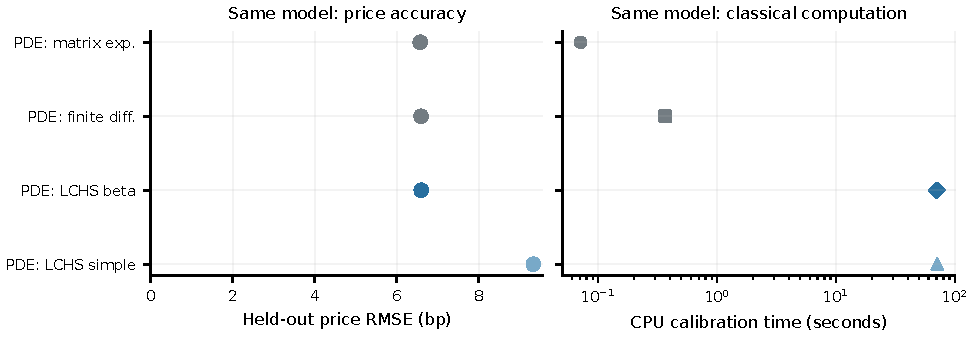
\includegraphics[width=.88\linewidth]{figures/solver_comparison.pdf}
\caption{Changing only the forward solver, $N=64$, out-of-family target with
5 bp price noise. Price RMSE is averaged within each dataset across five
starts, then across three datasets. Bars show dataset sample SD. CPU
calibration times exclude compilation and subsequent evaluation.}
\end{figure}
\section{Four-maturity smile and skew examples}
The main surface figure uses the positive quadratic family
\[
 a_s(x)=0.01+0.08\xi_{s1}+0.1\xi_{s2}(x+0.45)^2
                   +0.1\xi_{s3}(x-0.45)^2.
\]
The smile coefficients are $(0.10,0.50,0.50)$, $(0.16,0.50,0.50)$,
$(0.22,0.50,0.50)$ and $(0.28,0.50,0.50)$. The skew coefficients are
$(0.20,0.10,0.85)$, $(0.22,0.12,0.80)$, $(0.24,0.14,0.75)$ and
$(0.26,0.16,0.70)$. Intervals end at 0.25, 0.5, 0.75 and 1 year.
Each expiry contains quotes at normalised strikes
$0.70,0.78,0.87,0.95,1,1.06,1.15,1.28,1.40$.
These controlled examples illustrate two familiar shapes. They are neither
market observations nor additional independently measured quantum calibrations.

Exact 1,024-node propagation generates the reference prices. Sequential bounded
least squares fits three coefficients per interval on 128 nodes. Exact,
backward-Euler (1,024 substeps per interval) and beta-LCHS evaluations then use
the same fitted coefficients. LCHS uses 8,192 terms and cutoff 96. The explicit
tridiagonal spectral implementation is checked against dense matrix exponentials
on a small grid. Reference refinement is recorded in the validation JSON.
The two forward approximations are not separately refitted in this example.

All four maturity rows are independently propagated. The 3D mesh connects
these computed rows for display. The one-year panels compare the fine-grid
target, exact coarse-grid model, and LCHS model against the actual quotes.
The plotted price and IV arrays are exported to
\path{surface_examples/surface_plot_data.csv}. No price clipping or IV smoothing
is applied. Held-out price RMSE excludes the nine calibration strikes.

\section{Archived benchmark and additional diagnostics}
The supplementary benchmark figures retain the original four-cosine family.
Their numerical predictions and derivative checks are unchanged by the new
quadratic illustrative examples. Where an archived display interpolates between
its two quoted maturities, that display is not an additional calibration.

This supplement audits the supplied completed run \texttt{paper\_9684a7f0bec7}.
No original calibration was rerun. All 568 planned keys are accounted for.
567 completed runs and one failed AH input are retained. Errors below are
normalised prices multiplied by $10^4$ when labelled bp. Dataset standard
deviations are descriptive, not confidence intervals. Five initialisations
within one dataset do not constitute five independent market datasets.

\section{Comparisons and the missing AH input}
\begin{table}[htbp]\centering\caption{Held-out price RMSE at $N=64$ (normalised bp). Noisy columns average initialisations within each dataset, then datasets. The in-family AH noisy entry uses only two valid datasets.}\small
\begin{tabular}{lrrrr}\toprule Method & In, clean & In, noisy & Out, clean & Out, noisy\\\midrule
Exact expm & 1.078 & 1.913 $\pm$ 0.371 & 6.416 & 6.576 $\pm$ 0.135\\
FD + adjoint & 1.082 & 1.918 $\pm$ 0.366 & 6.438 & 6.596 $\pm$ 0.132\\
LCHS beta & 1.072 & 1.918 $\pm$ 0.369 & 6.446 & 6.602 $\pm$ 0.129\\
LCHS simple & 20.804 & 20.802 $\pm$ 0.251 & 9.283 & 9.335 $\pm$ 0.087\\
Andreasen--Huge & 0.351 & 2.726 $\pm$ 0.784 & 1.831 & 3.482 $\pm$ 0.067\\
PINN fixed & 1.303 & 1.734 $\pm$ 0.211 & 1.174 & 2.116 $\pm$ 0.054\\
PINN adaptive & 1.350 & 1.784 $\pm$ 0.251 & 1.143 & 2.062 $\pm$ 0.185\\
\bottomrule\end{tabular}\end{table}
In-family dataset 303 at noise level 5 bp contains a first-maturity call at
$k=0.7$ with observed value approximately 0.299932374, below intrinsic value 0.3.
Black implied volatility is undefined for this input and the AH baseline
stops. The quote is not clipped. Comparisons on this input do not have the
same feasibility conditions as the other datasets. The all-case table makes
the denominator difference explicit. The following table instead pairs the
same two feasible datasets for every method.
\begin{table}[htbp]\centering\caption{Paired feasible in-family noisy datasets (101 and 202), $N=64$. Held-out RMSE in normalised bp; sample SD over two datasets. Dataset 303 remains a separately reported failed-input stress case.}\small
\begin{tabular}{lrr}\toprule Method & Mean & Dataset SD\\\midrule
Exact expm & 1.712 & 0.184\\
FD + adjoint & 1.719 & 0.177\\
LCHS beta & 1.717 & 0.173\\
LCHS simple & 20.665 & 0.116\\
Andreasen--Huge & 2.726 & 0.784\\
PINN fixed & 1.660 & 0.236\\
PINN adaptive & 1.670 & 0.218\\
\bottomrule\end{tabular}\end{table}
\begin{figure}[H]\centering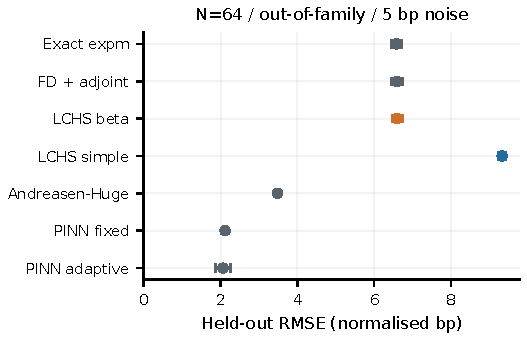
\includegraphics[width=.65\linewidth]{figures/heldout_comparison.pdf}
\caption{Out-of-family noisy case: means and sample SD across three independent
data seeds, after averaging five initialisations (AH deterministic).}\end{figure}

\section{Finite approximation and diagnostic scope}
All 240 finite-LCHS calibrations fail the full-domain butterfly and calendar
tests at price tolerance $10^{-8}$. For beta LCHS, only the $N=128$ butterfly
test also fails within the quote/test band (15 of 40 runs). Exact re-evaluation
passes at all 240 fitted designs. Full-grid details, maxima and band counts
are in \path{audit/arbitrage_by_method_grid.csv}. Per-run independently
reconstructed metrics are in \path{audit/independent_checks.csv}.
Both comparison kernels use $J=2048$ in calibration, but their cutoffs differ
(beta 48; simple 64). The forward sweep explicitly uses 16, 32 and 64.
The simple kernel has 4764 invalid held-out model IV evaluations among 43080.
Its conditional valid-IV RMSE must be accompanied by this coverage.
All reported ``certificate passes'' use measured error against exact
propagation at the same coefficients and are conditional perturbation tests.

\section{Quantisation, Fourier approximation and identifiability}
\begin{figure}[H]\centering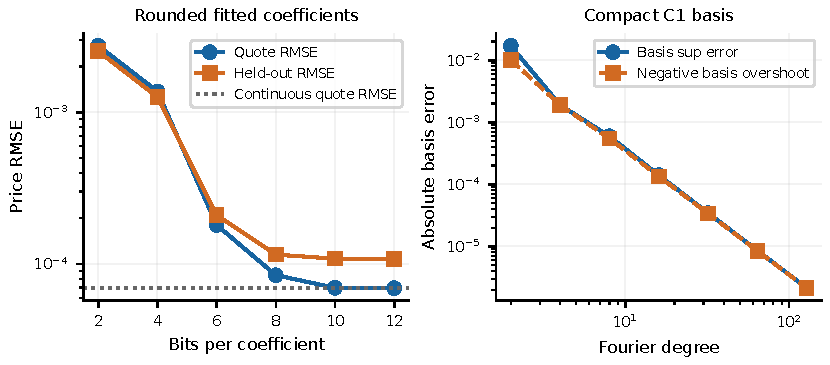
\includegraphics[width=.78\linewidth]{figures/precision_basis.pdf}
\caption{One-fit coefficient rounding and sampled Fourier diagnostics. The
Fourier panel evaluates one of four compactly supported basis functions on
4096 points. Its sampled maximum and derived illustrative budgets are not
continuous supremum certificates for all basis functions. No Fourier
approximation is used in the actual calibration.}\end{figure}
At four bits, training and held-out RMSE are 13.711 and 12.600 bp. The continuous
training fit is 0.693 bp. At ten and twelve bits, training errors are 0.696 and
0.693 bp. This is rounding without discrete re-optimisation on one fitted case.
The tested high-degree Fourier decay is consistent with algebraic convergence.
Neither an asymptotic rate proof nor polylogarithmic complexity follows.
\begin{figure}[H]\centering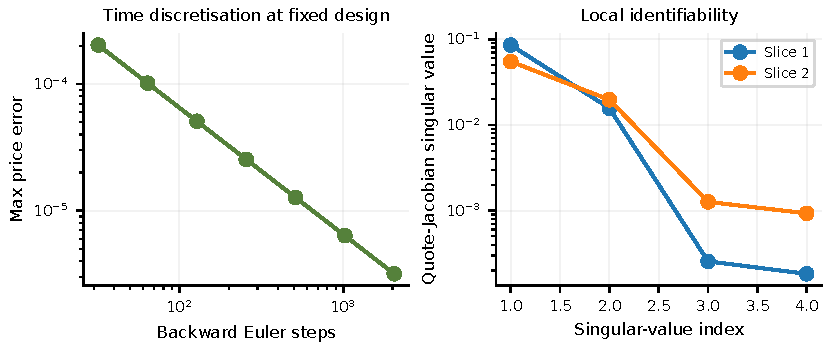
\includegraphics[width=.78\linewidth]{figures/fd_identifiability.pdf}
\caption{A fixed-design backward-Euler refinement diagnostic and local quote
Jacobian singular values for one selected exact fit.}\end{figure}
The maximum FD price error falls from $2.0279\times10^{-4}$ at 32 steps to
$6.3543\times10^{-6}$ at 1024 and $3.1773\times10^{-6}$ at 2048. This is a
fixed-design convergence check, not a recalibration at every time step count.
Jacobian condition numbers are about 467 and 59 for the two slices.

\section{Sensitivity experiments and confounders}
\begin{figure}[H]\centering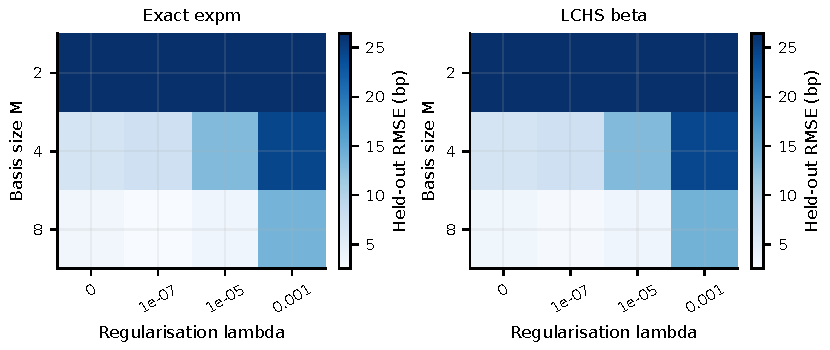
\includegraphics[width=.78\linewidth]{figures/ablation.pdf}
\caption{Basis-family and regularisation sensitivity on one noisy out-of-family
dataset and one initialisation. Centres and widths change with $M$, so the
bases are not nested. The second-difference penalty is absent for $M=2$ by
definition. This is not a validation-selected performance estimate.}\end{figure}
At $M=8$, $\lambda=10^{-7}$, exact and beta held-out errors are about 2.50 and
2.77 bp. A prospective model comparison must select $M,\lambda$ using training
and validation information and assess a fresh test set. The present inspected
held-out set cannot serve as an untouched confirmatory test for that choice.
\begin{figure}[H]\centering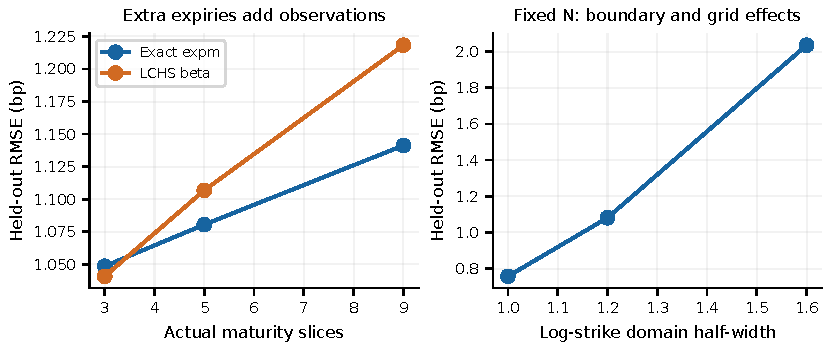
\includegraphics[width=.78\linewidth]{figures/domain_slices.pdf}
\caption{Domain and slice sensitivities. Fixed spatial node count means that
changing the domain changes spacing. Nominal 2, 4 and 8 slice experiments
insert the true change point, giving 3, 5 and 9 actual slices and 21, 35 and
63 quotes. They change both model/time resolution and available observations.}\end{figure}

\section{Neural and quantum diagnostics}
\begin{figure}[H]\centering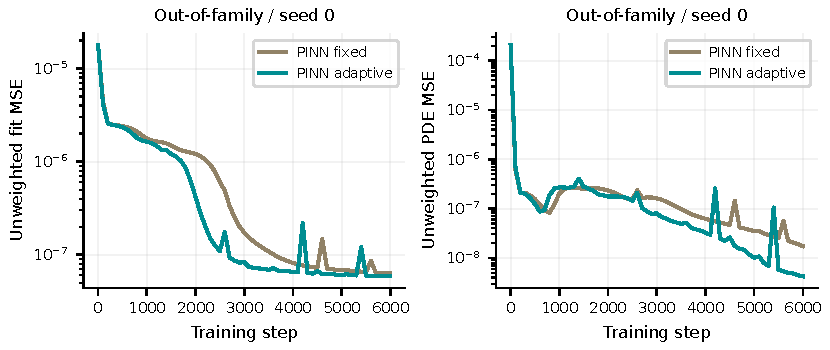
\includegraphics[width=.78\linewidth]{figures/pinn_losses.pdf}
\caption{Fixed/adaptive PINN training diagnostics. The comparator is a
documented adaptation with a fixed 6000-epoch budget. It is not an exact
reproduction of the original Whack-a-Mole implementation.}\end{figure}
Neither neural model has a counted common-grid butterfly/calendar failure in
its 40 completed runs. This sampled result is not a structural guarantee over
all strikes and maturities. Fixed-epoch completion is not optimiser convergence.
\begin{figure}[H]\centering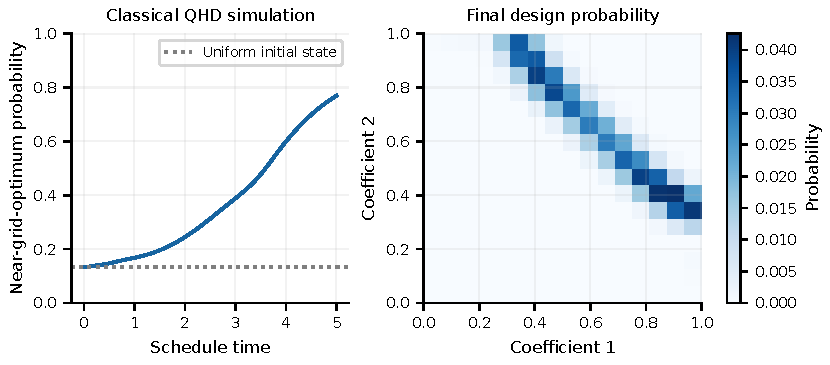
\includegraphics[width=.78\linewidth]{figures/qhd_diagnostics.pdf}
\caption{QHD-inspired split-step evolution on a classically tabulated 256-point
landscape, with a separate 1500-versus-3000-step refinement check. The coherent
circuit evaluates only four corner designs.}\end{figure}
The near-minimum criterion is within one per cent of the finite loss range.
Probability rises from 13.28\% to 76.92\%. The refined distribution differs in
total variation by $8.46\times10^{-7}$. These observations do not imply
continuous global optimality or quantum advantage.

\section{Reproduction and provenance}
The companion \texttt{surface\_calibration\_experiments.ipynb} runs the new
four-maturity surface examples and measured calibration, checks circuits and regenerates figures and
TeX. It embeds the immutable archived evidence and verifies its hash before
use. The independent audit reads saved predictions without executing code
from that evidence. The optional original full experiment notebook reruns
the larger numerical benchmark. These execution scopes are kept separate.
Original raw observations, checkpoints, CSV diagnostics and source code are
retained under \texttt{paper/evidence/} in the repository
\url{https://github.com/khoshisashi/quantum-local-vol}. No market observations
were supplied. Runtime versions and CPU backend are in the original manifest.
The submitted input ZIP has SHA-256
\par\noindent\texttt{6684a5cf912b9703b9180395bb1df48e832}\newline
\texttt{fcc5944610421d279a211952b4fca} (concatenate the two lines).

\footnotesize
\begin{thebibliography}{99}
\setlength{\itemsep}{0pt}
\bibitem{lchs} D. An, J.-P. Liu, and L. Lin, ``Linear combination of Hamiltonian simulation for nonunitary dynamics with optimal state preparation cost,'' \emph{Physical Review Letters}, vol. 131, no. 15, Art. no. 150603, 2023, doi: \href{https://doi.org/10.1103/PhysRevLett.131.150603}{10.1103/PhysRevLett.131.150603}.
\bibitem{nearoptimal} D. An, A. M. Childs, and L. Lin, ``Quantum algorithm for linear non-unitary dynamics with near-optimal dependence on all parameters,'' \emph{Communications in Mathematical Physics}, vol. 407, Art. no. 19, 2026, doi: \href{https://doi.org/10.1007/s00220-025-05509-w}{10.1007/s00220-025-05509-w}.
\bibitem{yano} H. Yano and Y. Sato, ``Quantum framework for parameterizing partial differential equations via diagonal block-encoding,'' arXiv preprint \href{https://arxiv.org/abs/2603.01358v1}{arXiv:2603.01358v1}, 2026.
\bibitem{qhd} J. Leng, E. Hickman, J. Li, and X. Wu, ``Quantum Hamiltonian descent,'' arXiv preprint \href{https://arxiv.org/abs/2303.01471v1}{arXiv:2303.01471v1}, 2023.
\bibitem{sato} Y. Sato, J. Kato, H. Yano, K. Ito, and N. Yamamoto, ``Explicit block-encoding for partial differential equation-constrained optimization,'' arXiv preprint \href{https://arxiv.org/abs/2511.14420v2}{arXiv:2511.14420v2}, 2026.
\end{thebibliography}

\end{document}
